% arara: xelatex: {shell: true}
% arara: xelatex: {shell: true}
%\documentclass[czech,aspectratio=169,xcolor={table}]{beamer}
\documentclass[czech,xcolor={table}]{beamer}
\usepackage[orientation=landscape,size=custom,width=16,height=9,scale=0.5,debug]{beamerposter} 
%\usepackage[czech]{babel}
\usepackage[czech]{babel}

\usepackage{polyglossia}
\setmainlanguage{czech}

% https://hartwork.org/beamer-theme-matrix/
\usetheme[compress]{Singapore}
\usecolortheme{default}
\useinnertheme{circles} % rectangles circles inmargin rounded

\definecolor{CVUT}{HTML}{0065BD}


%\setbeamertemplate{footline}[frame number]
\setbeamercolor*{structure}{bg=white,fg=CVUT}
\setbeamercovered{transparent}
\setbeamertemplate{footline}[frame number]

\usepackage{colortbl}
\usepackage{fontspec}
\usepackage{setspace}
\usepackage{relsize}
\usepackage{tabularx}
\usepackage{amsmath} %advanced maths
\usepackage{amssymb} %additional math symbols
\usepackage{array}
\usepackage{multirow}
\usepackage{multicol}
\usepackage{rotating}
\usepackage{minted}
%\usepackage{microtype}
%\setsansfont{Technika-Book}
%\setmonofont[Scale=.95]{DejaVu Sans Mono}

\beamertemplatenavigationsymbolsempty
\definecolor{highlite}{RGB}{255, 255, 0}

\usepackage{graphicx}
%\usepackage{minted}
\usepackage{hyperref}
\usepackage{booktabs}
\usepackage{appendixnumberbeamer}

\usepackage{regexpatch}
\makeatletter
% Change the `-` delimiter to an active character
\xpatchparametertext\@@@cmidrule{-}{\cA-}{}{}
\xpatchparametertext\@cline{-}{\cA-}{}{}
\makeatother

\title{Urban Data Visualization}
\author{Vojtěch Tomas}
\date{}
%\titlegraphic{\includegraphics[width=.2\textwidth]{fit}}

\begin{document}

	\begin{frame}
		\titlepage
		\begin{center}
		Supervisor: Ing. David Sedláček, Ph.D. \\\vspace{1em}
		\small Department of Computer Graphics and Interaction  --- Computer Graphics
		\end{center}
	\end{frame}

	\section{Introduction}
	\begin{frame}
		\frametitle{Assignment}
		{
			\centering
			Design a \textit{usefull} urban data visualization tool\\\vspace{1em}
		}
		\textbf{Assignment}
		\begin{itemize}
			\item urban data visualization 
			\item coopeartion with IPR Prague and CAMP
		\end{itemize}
		\textbf{Goals}
		\begin{itemize}
			\item streamline urban data visualization pipeline
			\item enable the production of physical models of urban areas
			\item support for visualization projection mapping
		\end{itemize}
	\end{frame}


	\begin{frame}
		\frametitle{Motivation}
		{
			\begin{center}
				\textbf{Urban environment} exists when a sustained stream of \textbf{people} occupies it. 
			\end{center}
		}
		\begin{center}
			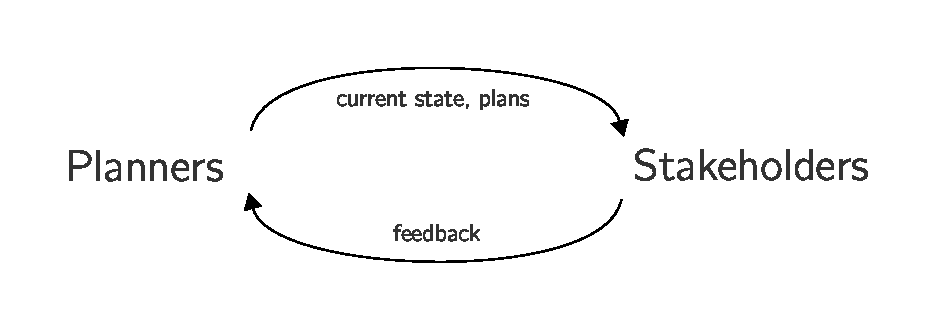
\includegraphics[width=0.7\textwidth]{imgs/Loop1.pdf}
		\end{center}
		{
			\begin{center}
				\textbf{People} generate \textbf{data}
			\end{center}
		}
	\end{frame}

	\begin{frame}
		\frametitle{Motivation}
		{
			\begin{center}
			a \textbf{society} --- \textbf{data} --- \textbf{model} --- \textbf{development} loop
			\end{center}
		}
		\begin{center}
			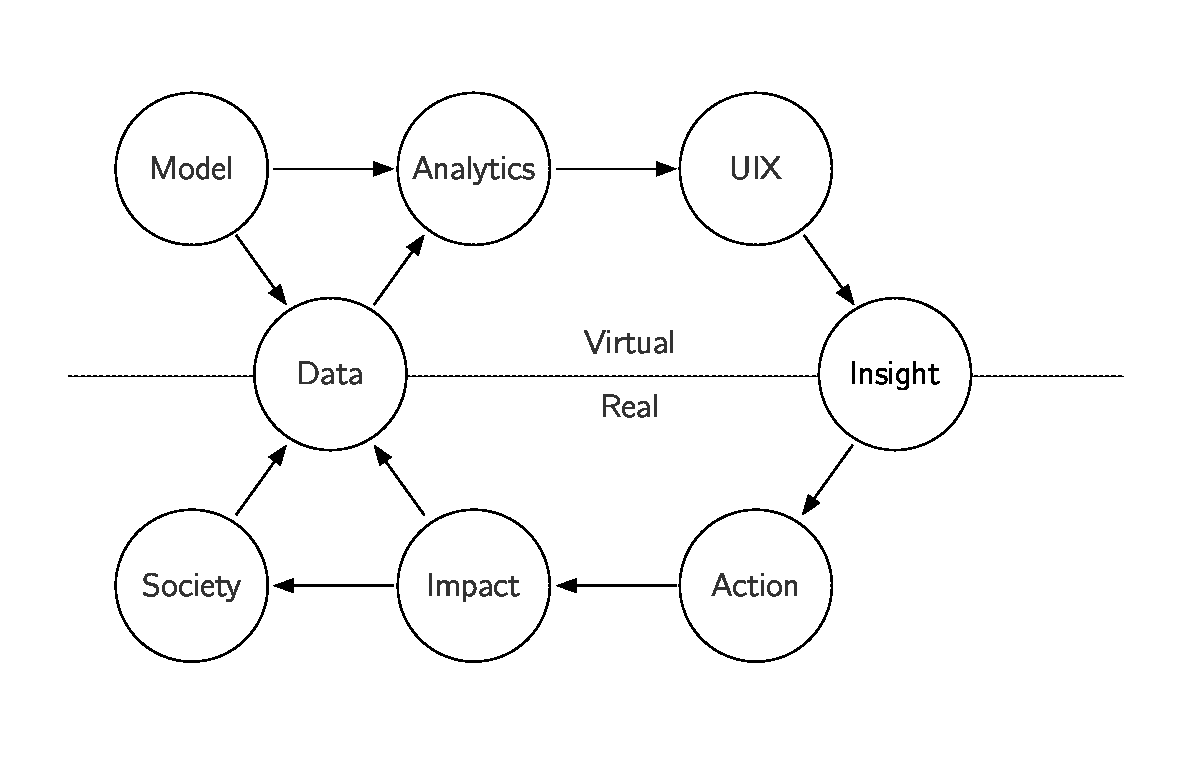
\includegraphics[width=0.6\textwidth]{imgs/Loop2.pdf}
		\end{center}
		\vspace{1em}
		\tiny Image sources [1]
	\end{frame}

	\begin{frame}
		\frametitle{Urban Data Visualization}
		\textbf{Why bother visualizing urban data?}
		\begin{itemize}
			\item streamline city planning
			\item data accessibility for real-estate developers and architects
			\item information platform for general public 
		\end{itemize}
	\end{frame}

	%%%%%%%%%%%%%%%%%%%%

	\section{State of the Art}
	\begin{frame}
		\frametitle{Urban Data}
		\begin{columns}[t]
			\begin{column}{0.5\textwidth}
				\textbf{Sources}
				\begin{itemize}
					\item Administrations (Open data)
					\item Ubicomp --- mobile phones, sensors, workstations\ldots
				\end{itemize}
			\end{column}
			\begin{column}{0.45\textwidth}
				\textbf{Formats}
				\begin{itemize}
					\item Web-friendly formats\\ 
					CityGML, CityJSON, GeoJSON
					\item Future-proofing\\ 
					BIM and IFC
				\end{itemize}
			\end{column}
		\end{columns}
	\end{frame}

	\begin{frame}
		\frametitle{Existing solutions}
		\begin{center}
			Physical components vs virtual environmetns
		\end{center}
		\begin{columns}[t]
			\begin{column}{0.5\textwidth}
				\textbf{Virtual envronments}
				\begin{itemize}
					\item ArcGIS, QGIS
					\item UBER - kepler.gl, Movement
					\item Cesium
					\item Game Engines
				\end{itemize}
			\end{column}
			\begin{column}{0.45\textwidth}
				\textbf{Physical installations}
				\begin{itemize}
					\item Tactile Matrix
					\item CAMP Exhibitions 
						\begin{itemize}
							\item Rohanský ostrov: nový Karlín?
						\end{itemize}
				\end{itemize}
			\end{column}
		\end{columns}
		
	\end{frame}


	\begin{frame}
		\frametitle{Tactile Matrix}
		\begin{columns}
			\begin{column}{0.6\textwidth}
				\begin{center}
					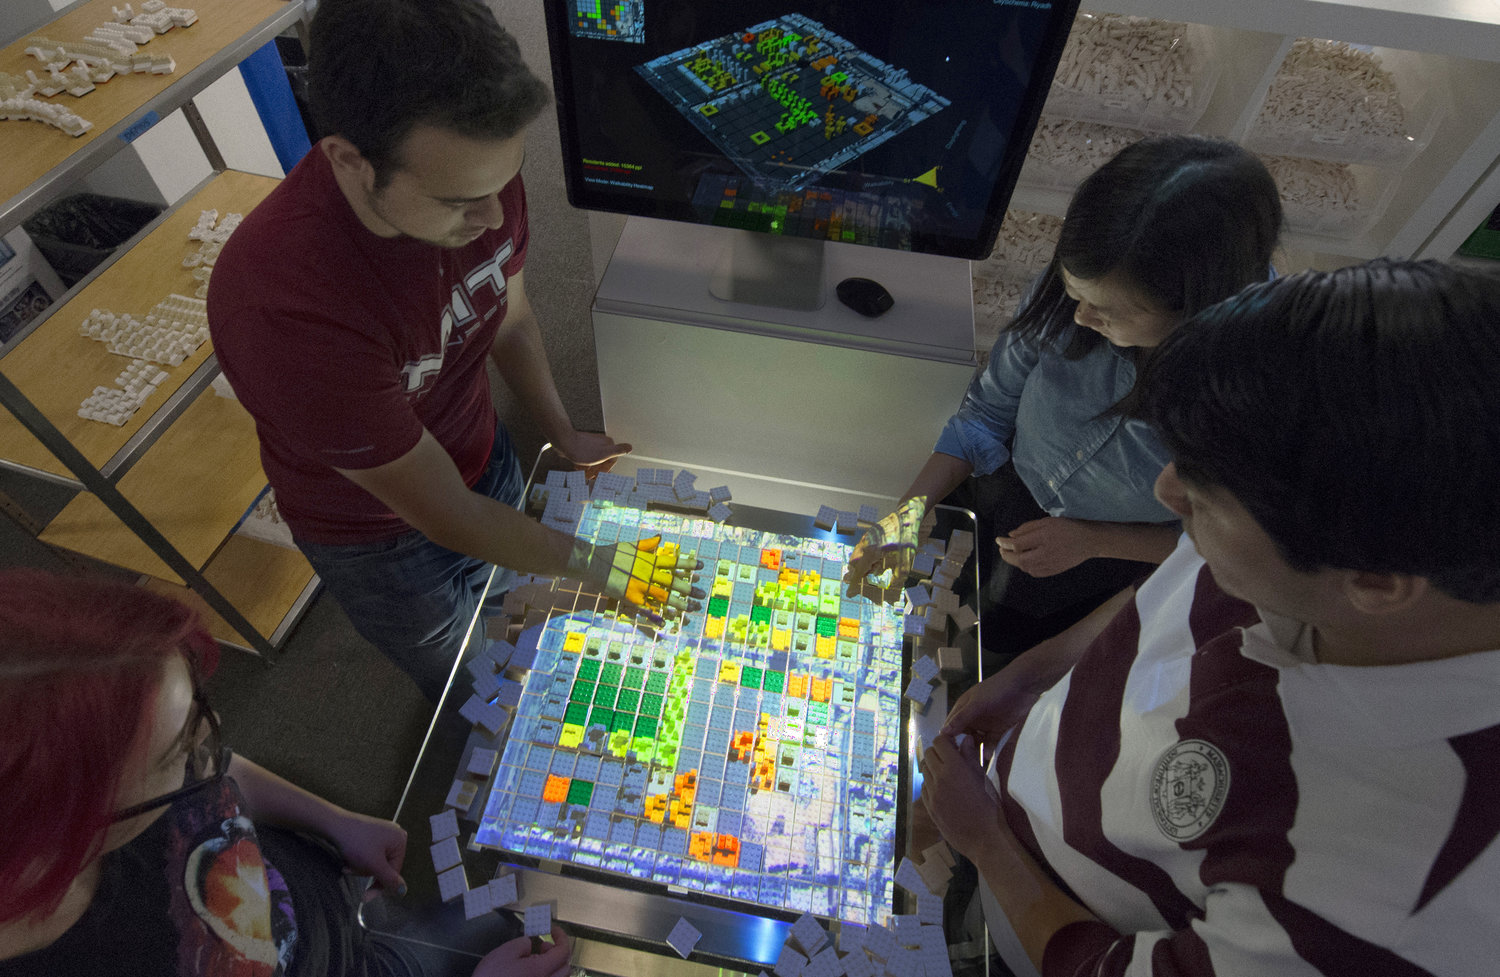
\includegraphics[width=1\textwidth]{imgs/tactile.jpg}
				\end{center}
			\end{column}
			\begin{column}{0.45\textwidth}
				\begin{center}
					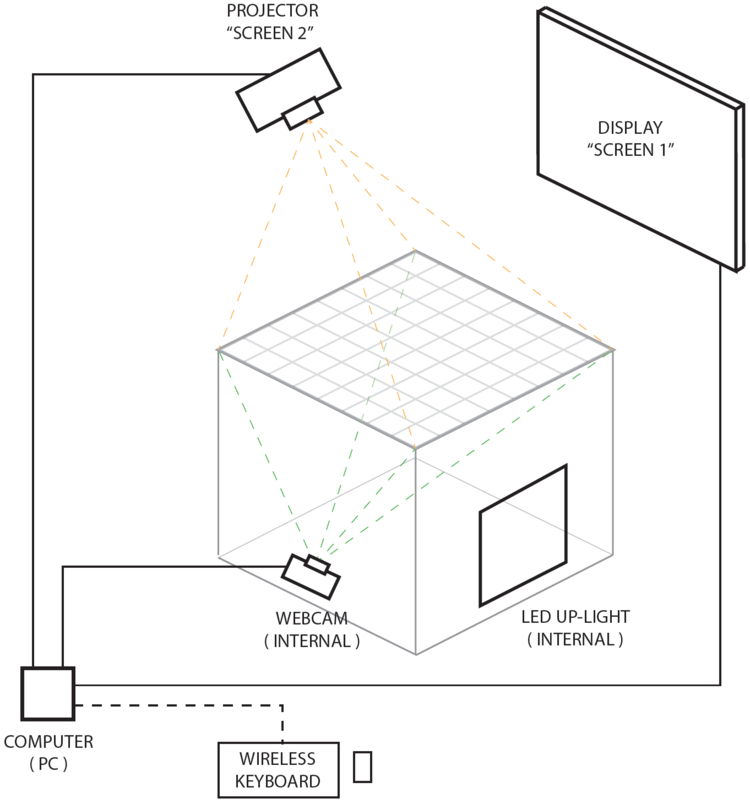
\includegraphics[width=0.7\textwidth]{imgs/tactilematrixelectronics.png}
				\end{center}
			\end{column}
		\end{columns}	
		\vspace{1em}
		\tiny Image sources [2] and [3]
	\end{frame}

	\begin{frame}
		\frametitle{Rohanský ostrov: nový Karlín?}
		\begin{columns}
			\begin{column}{0.5\textwidth}
				\begin{center}
					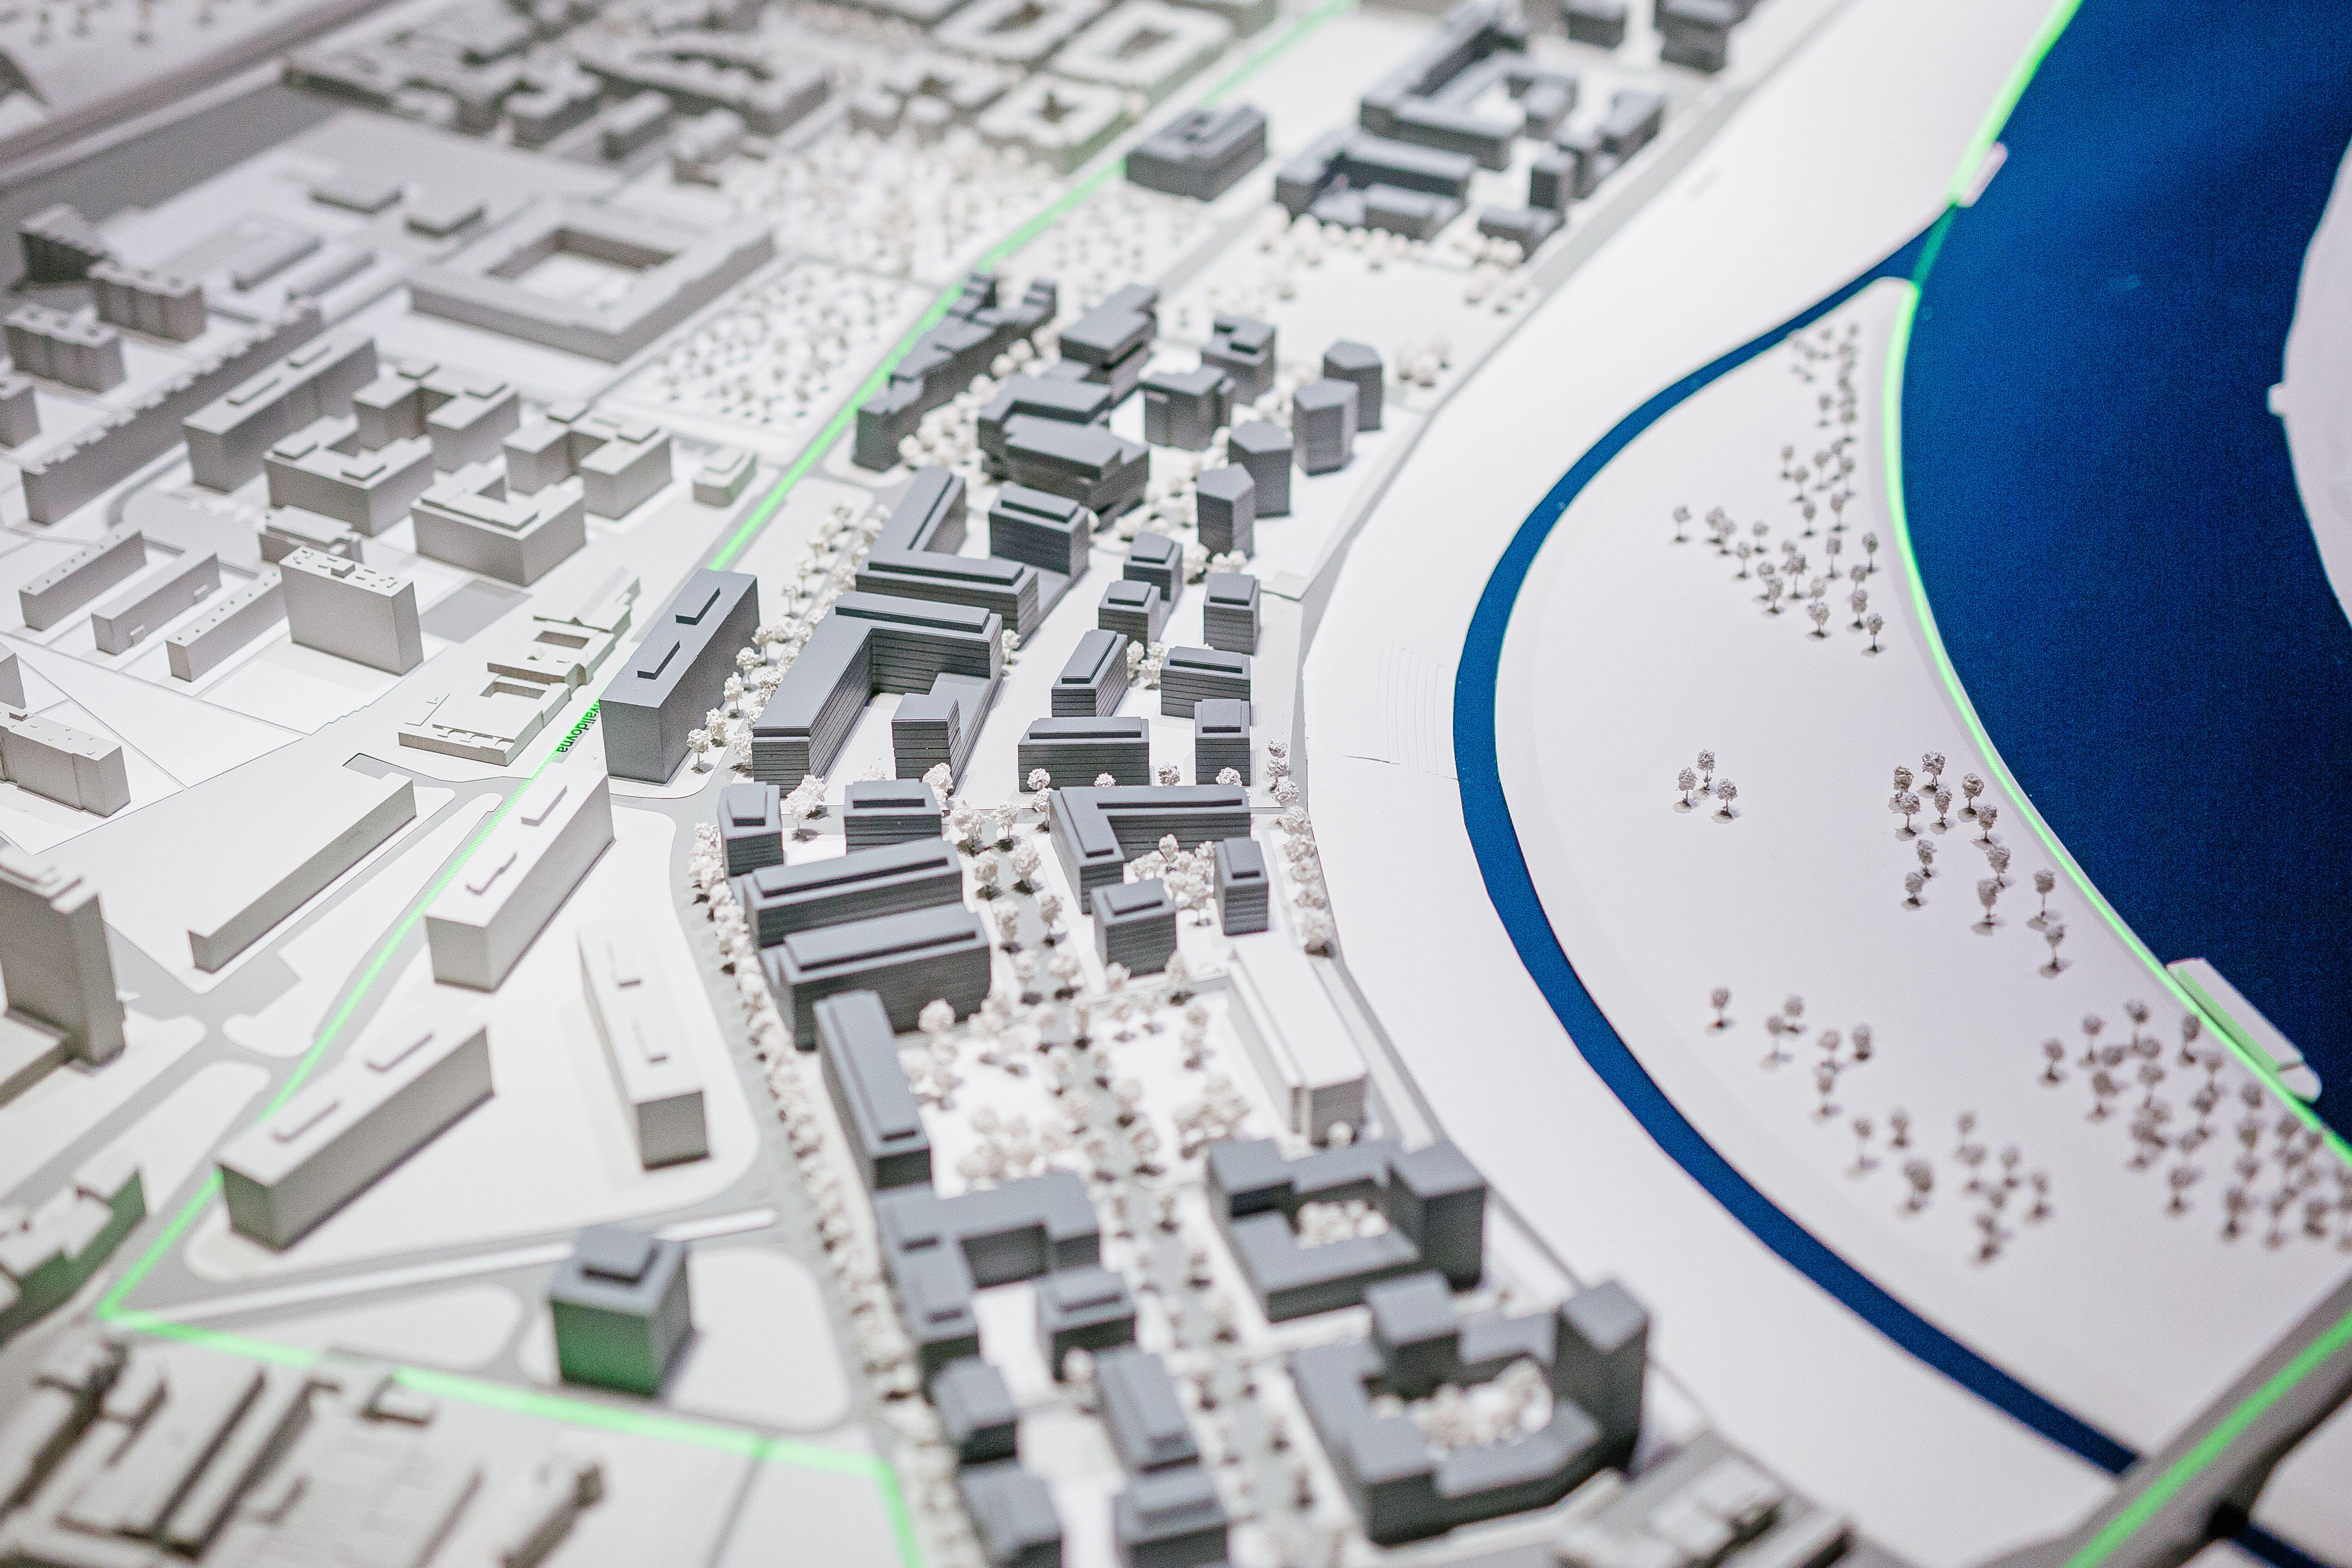
\includegraphics[width=1\textwidth]{imgs/rohan1.jpg}
				\end{center}
			\end{column}
			\begin{column}{0.5\textwidth}
				\begin{center}
					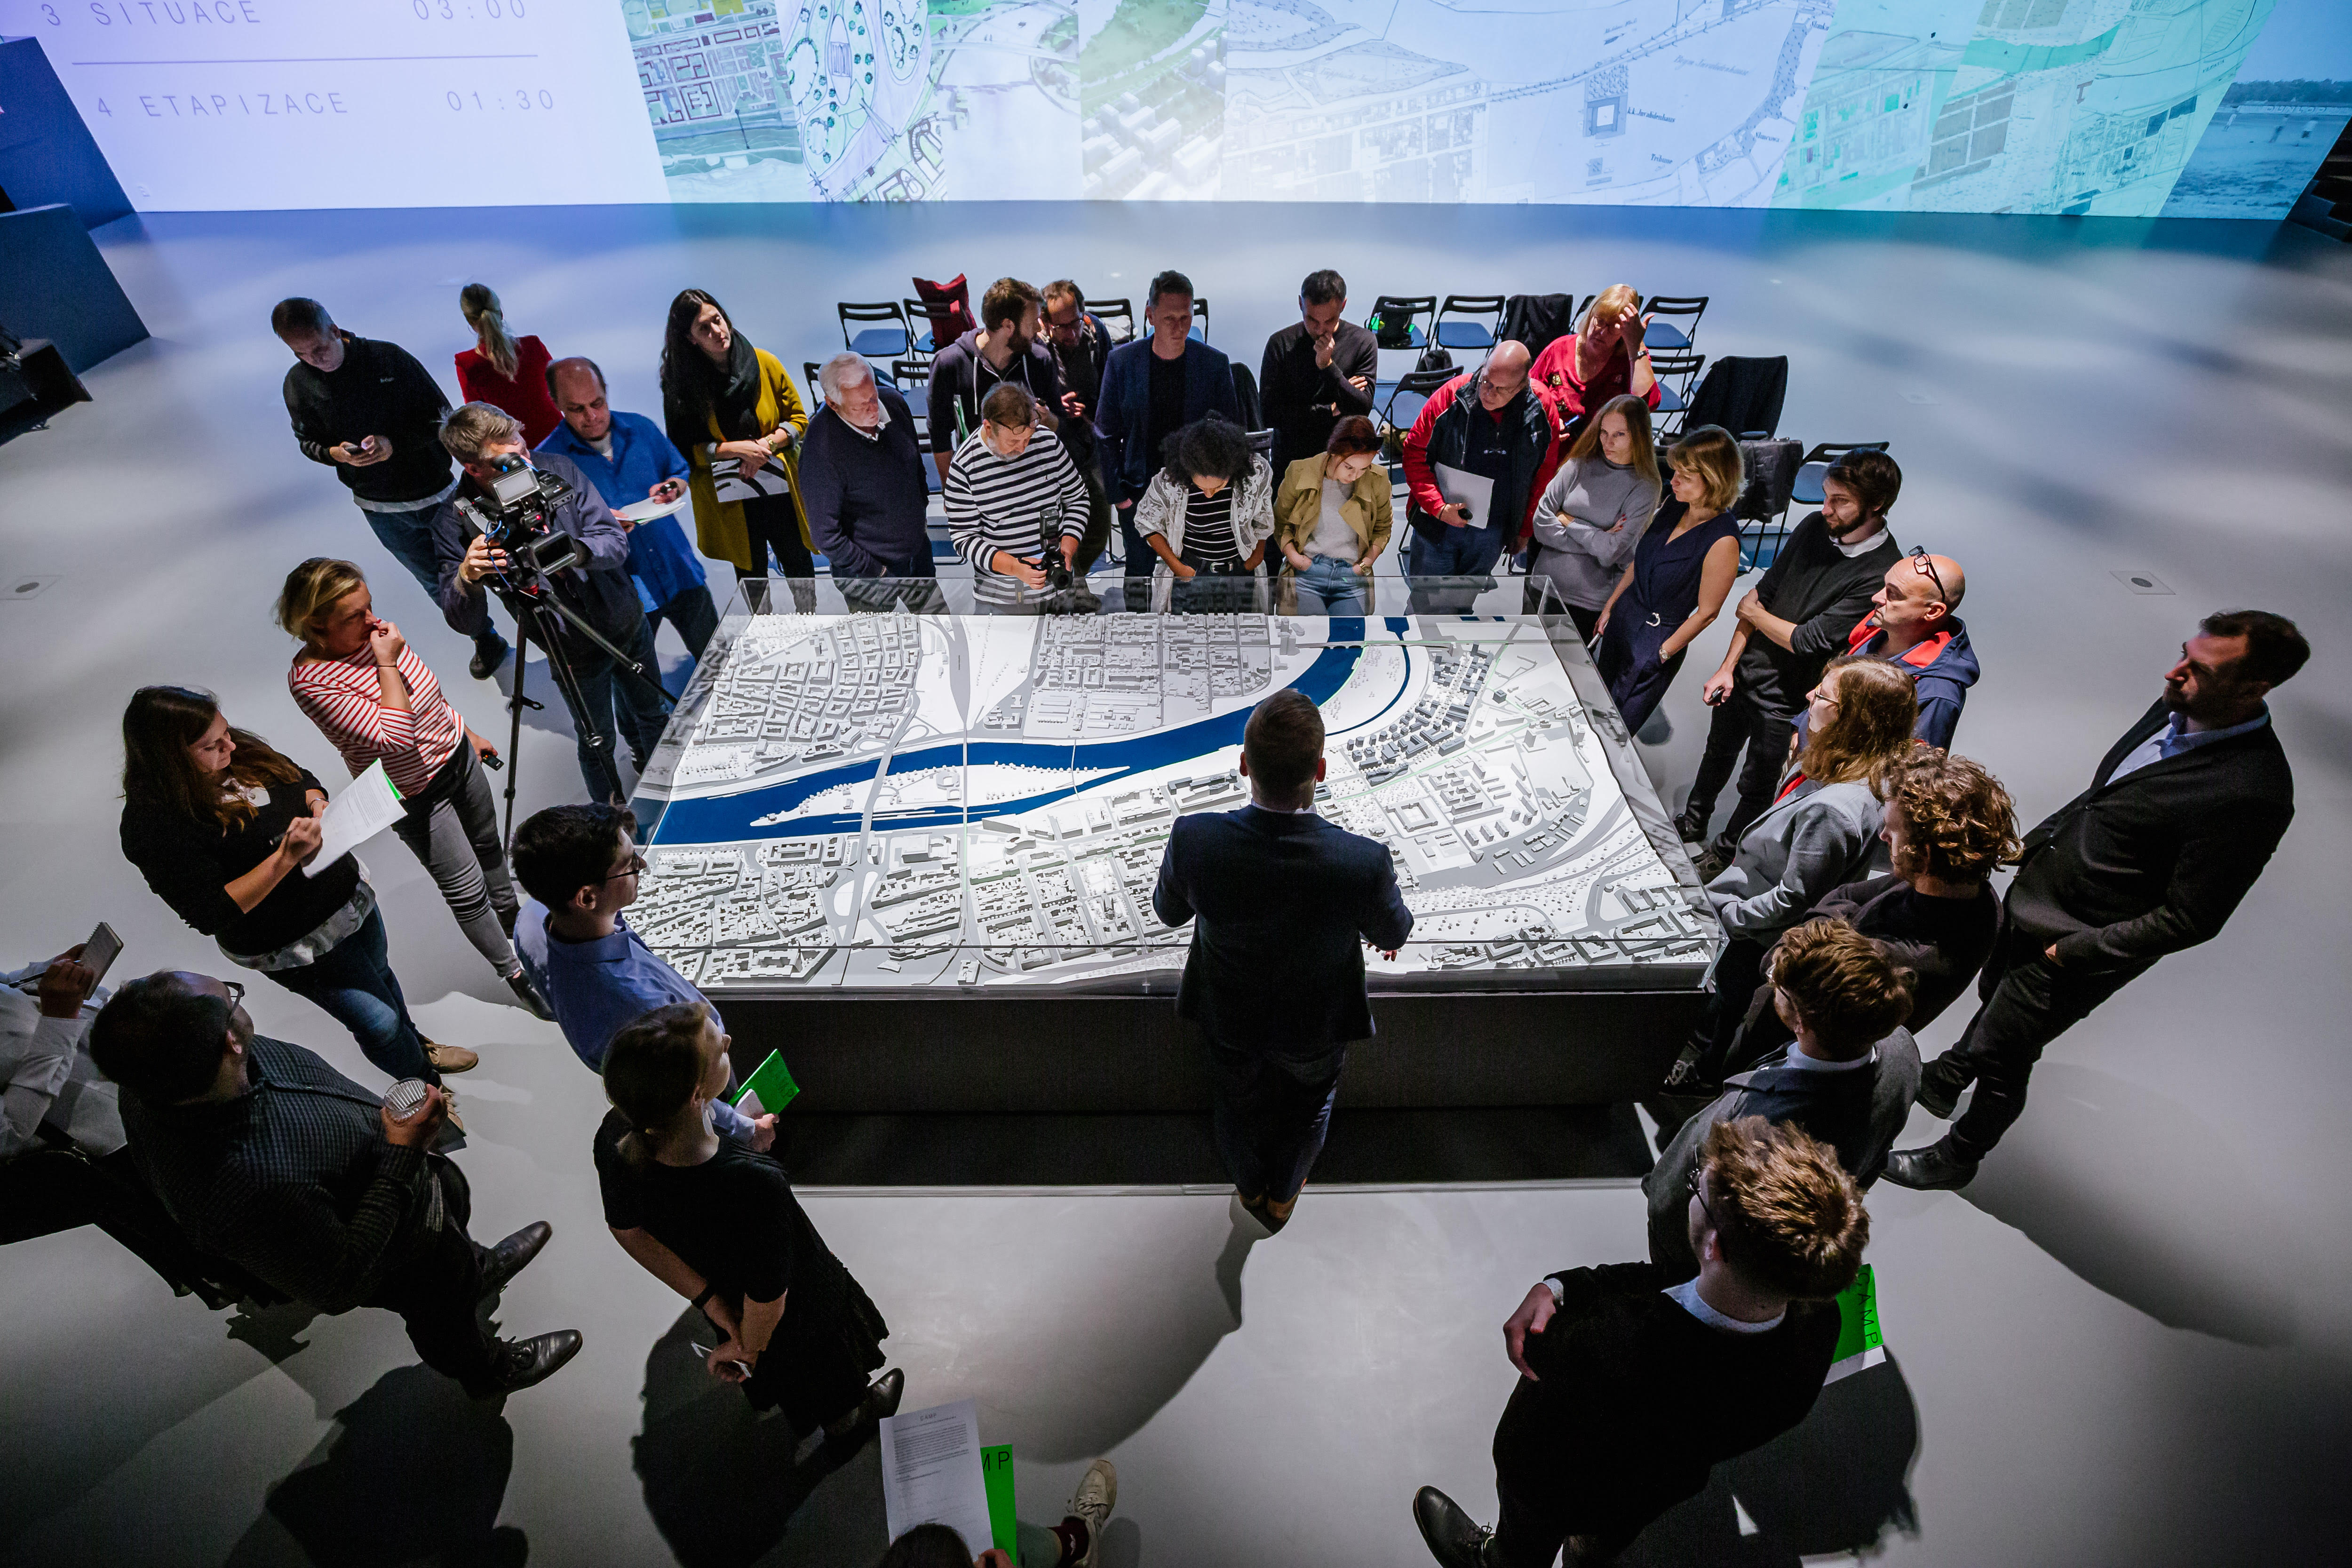
\includegraphics[width=1\textwidth]{imgs/rohan3.jpg}
				\end{center}
			\end{column}
		\end{columns}	
		\vspace{1em}
		\tiny Image sources [4]
	\end{frame}

	%%%%%%%%%%%%%%%%%%%%

	\section{Design and POC}

	\begin{frame}
		\frametitle{Design}
		\textbf{Virtual components}
		\begin{itemize}
			\item modular data processing backend 
			\item editor for urban data mapping
			\item IO for physical models
		\end{itemize}
		\textbf{Physical components}
		\begin{itemize}
			\item LEGO or 3D printed city tiles
			\item projection mapping system
		\end{itemize}
		\textbf{Outputs}
		\begin{itemize}
			\item virtual view + projection mapping view
			\item data for physical model assembly
		\end{itemize}
	\end{frame}

	\begin{frame}
		\frametitle{}
		\begin{center}
			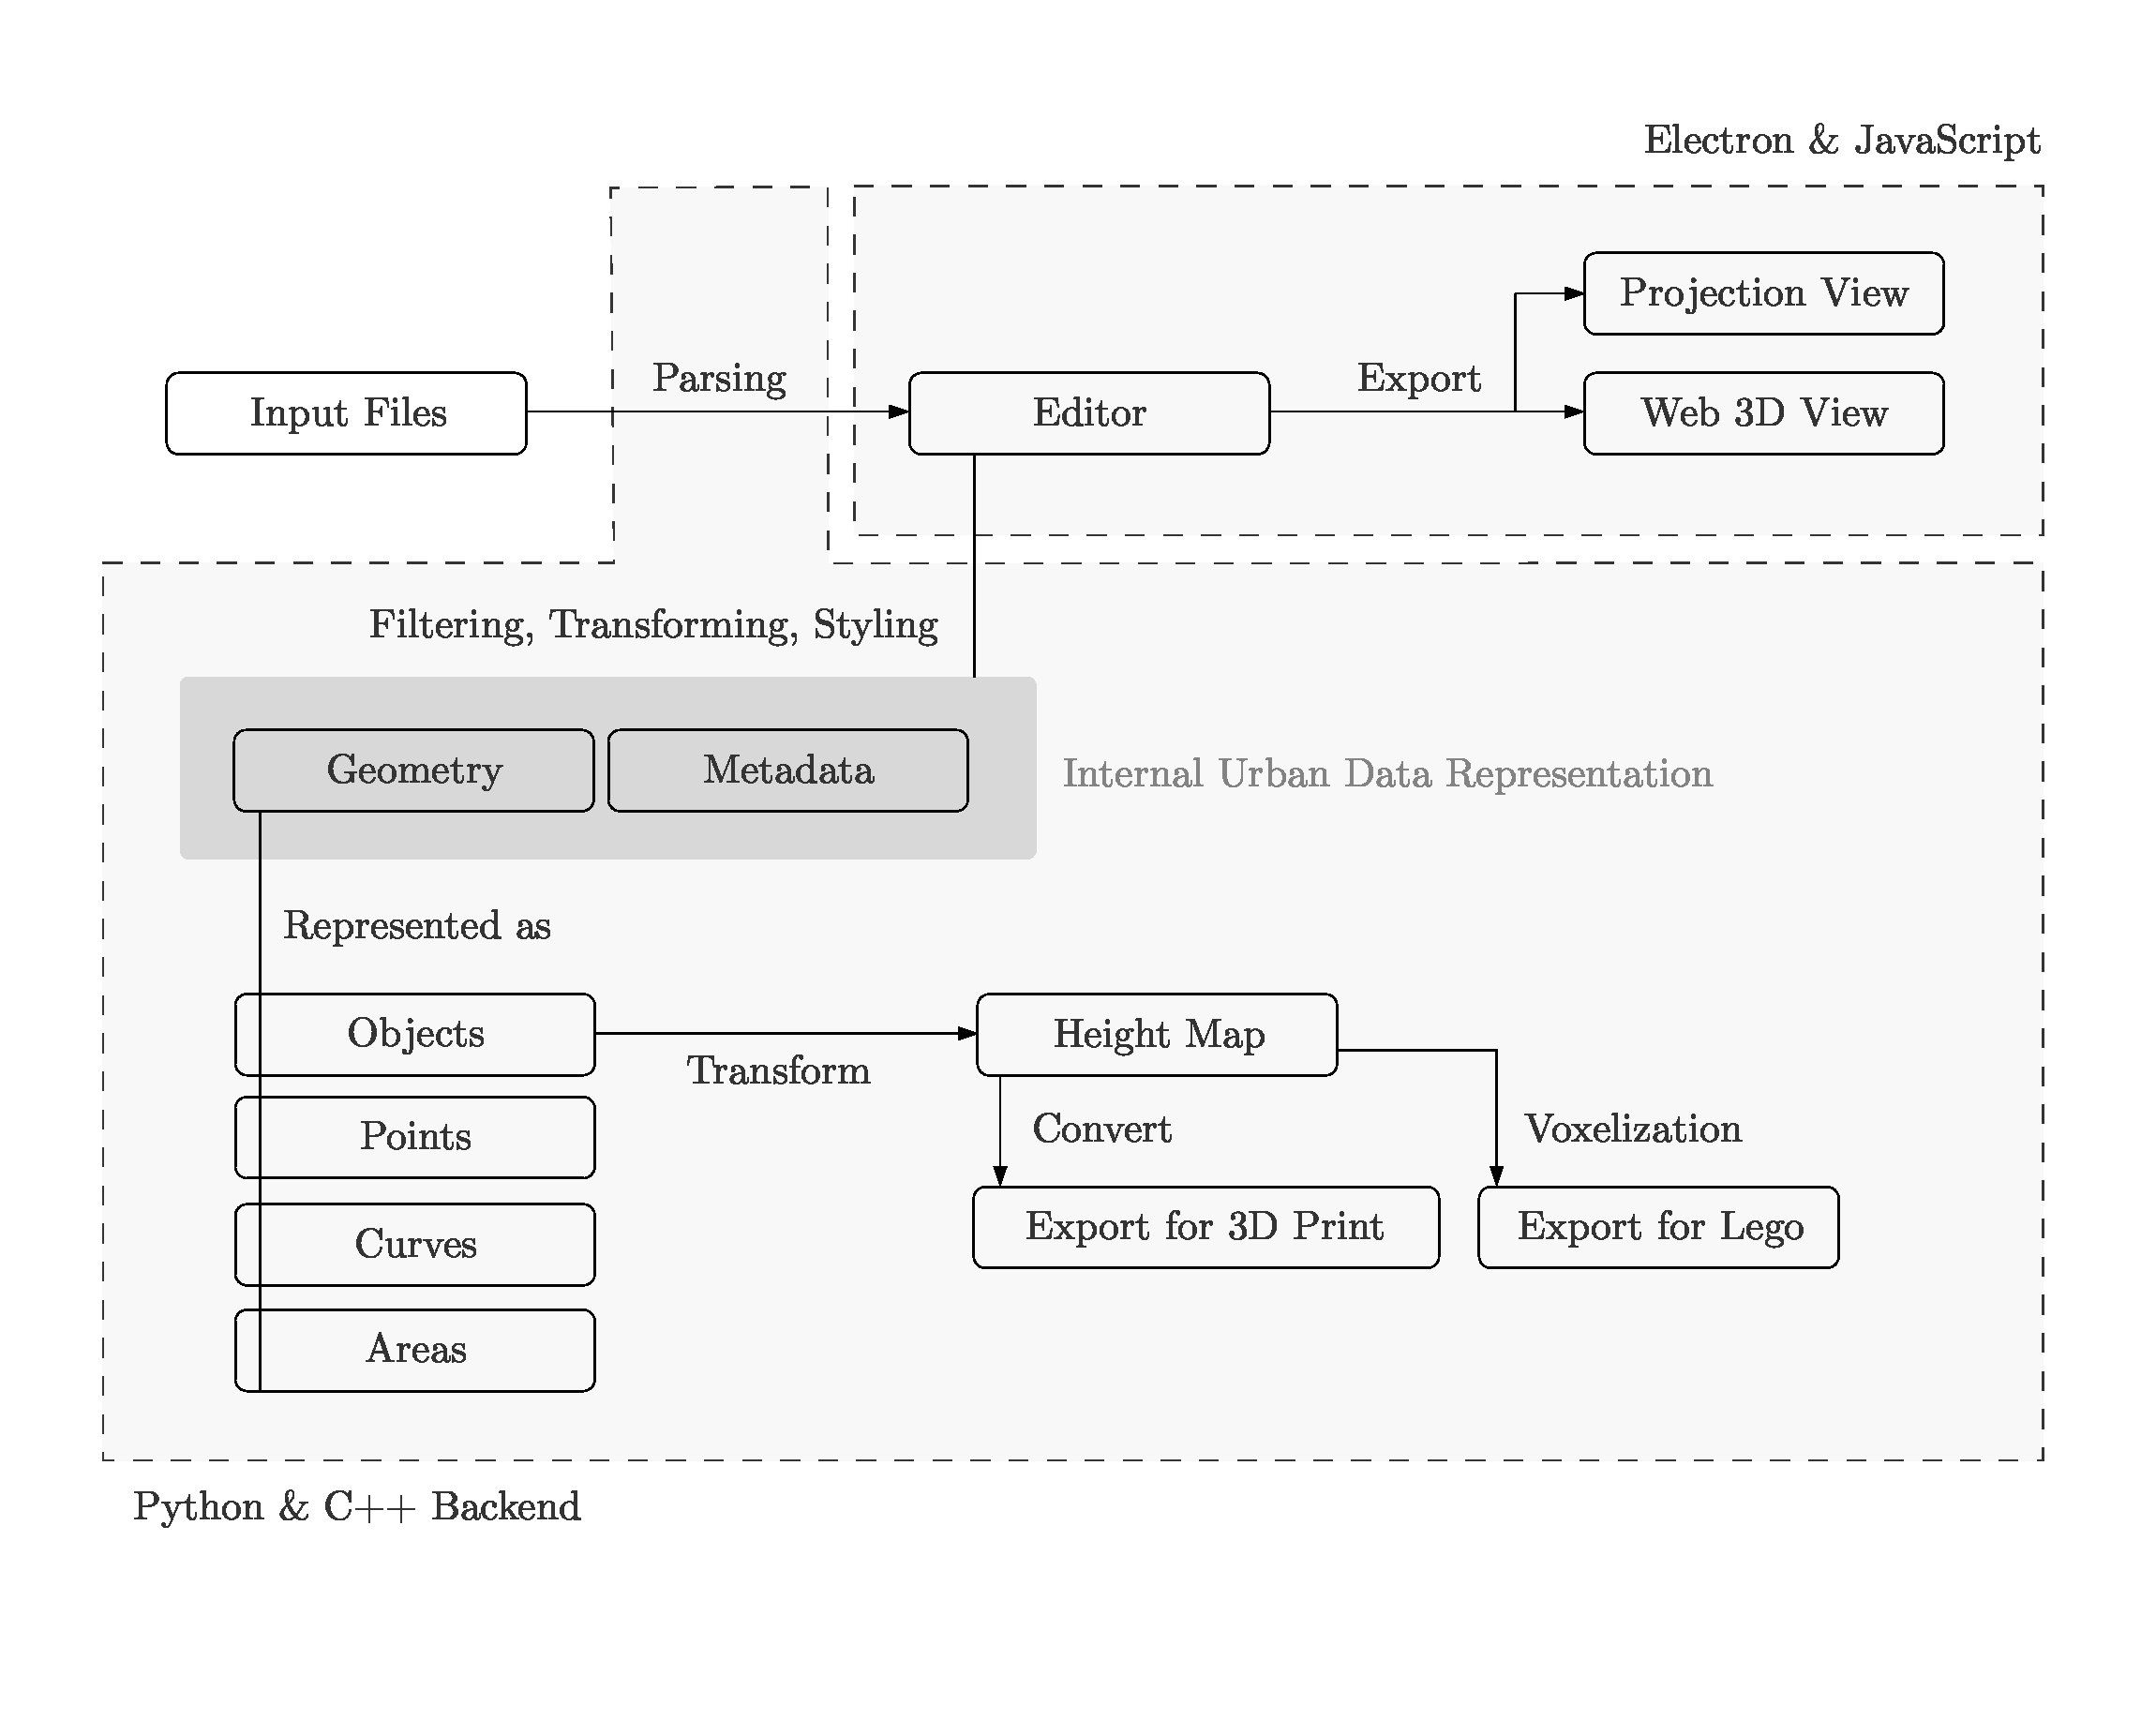
\includegraphics[width=0.75\textwidth]{imgs/app.pdf}
		\end{center}
	\end{frame}

	\begin{frame}
		\frametitle{POC}

		\begin{itemize}
			\item Web visualization of Urban Data
			\item Electron-based visual programming editor with Python backend
		\end{itemize}
	\end{frame}

	\begin{frame}
		\frametitle{}
		\begin{center}
			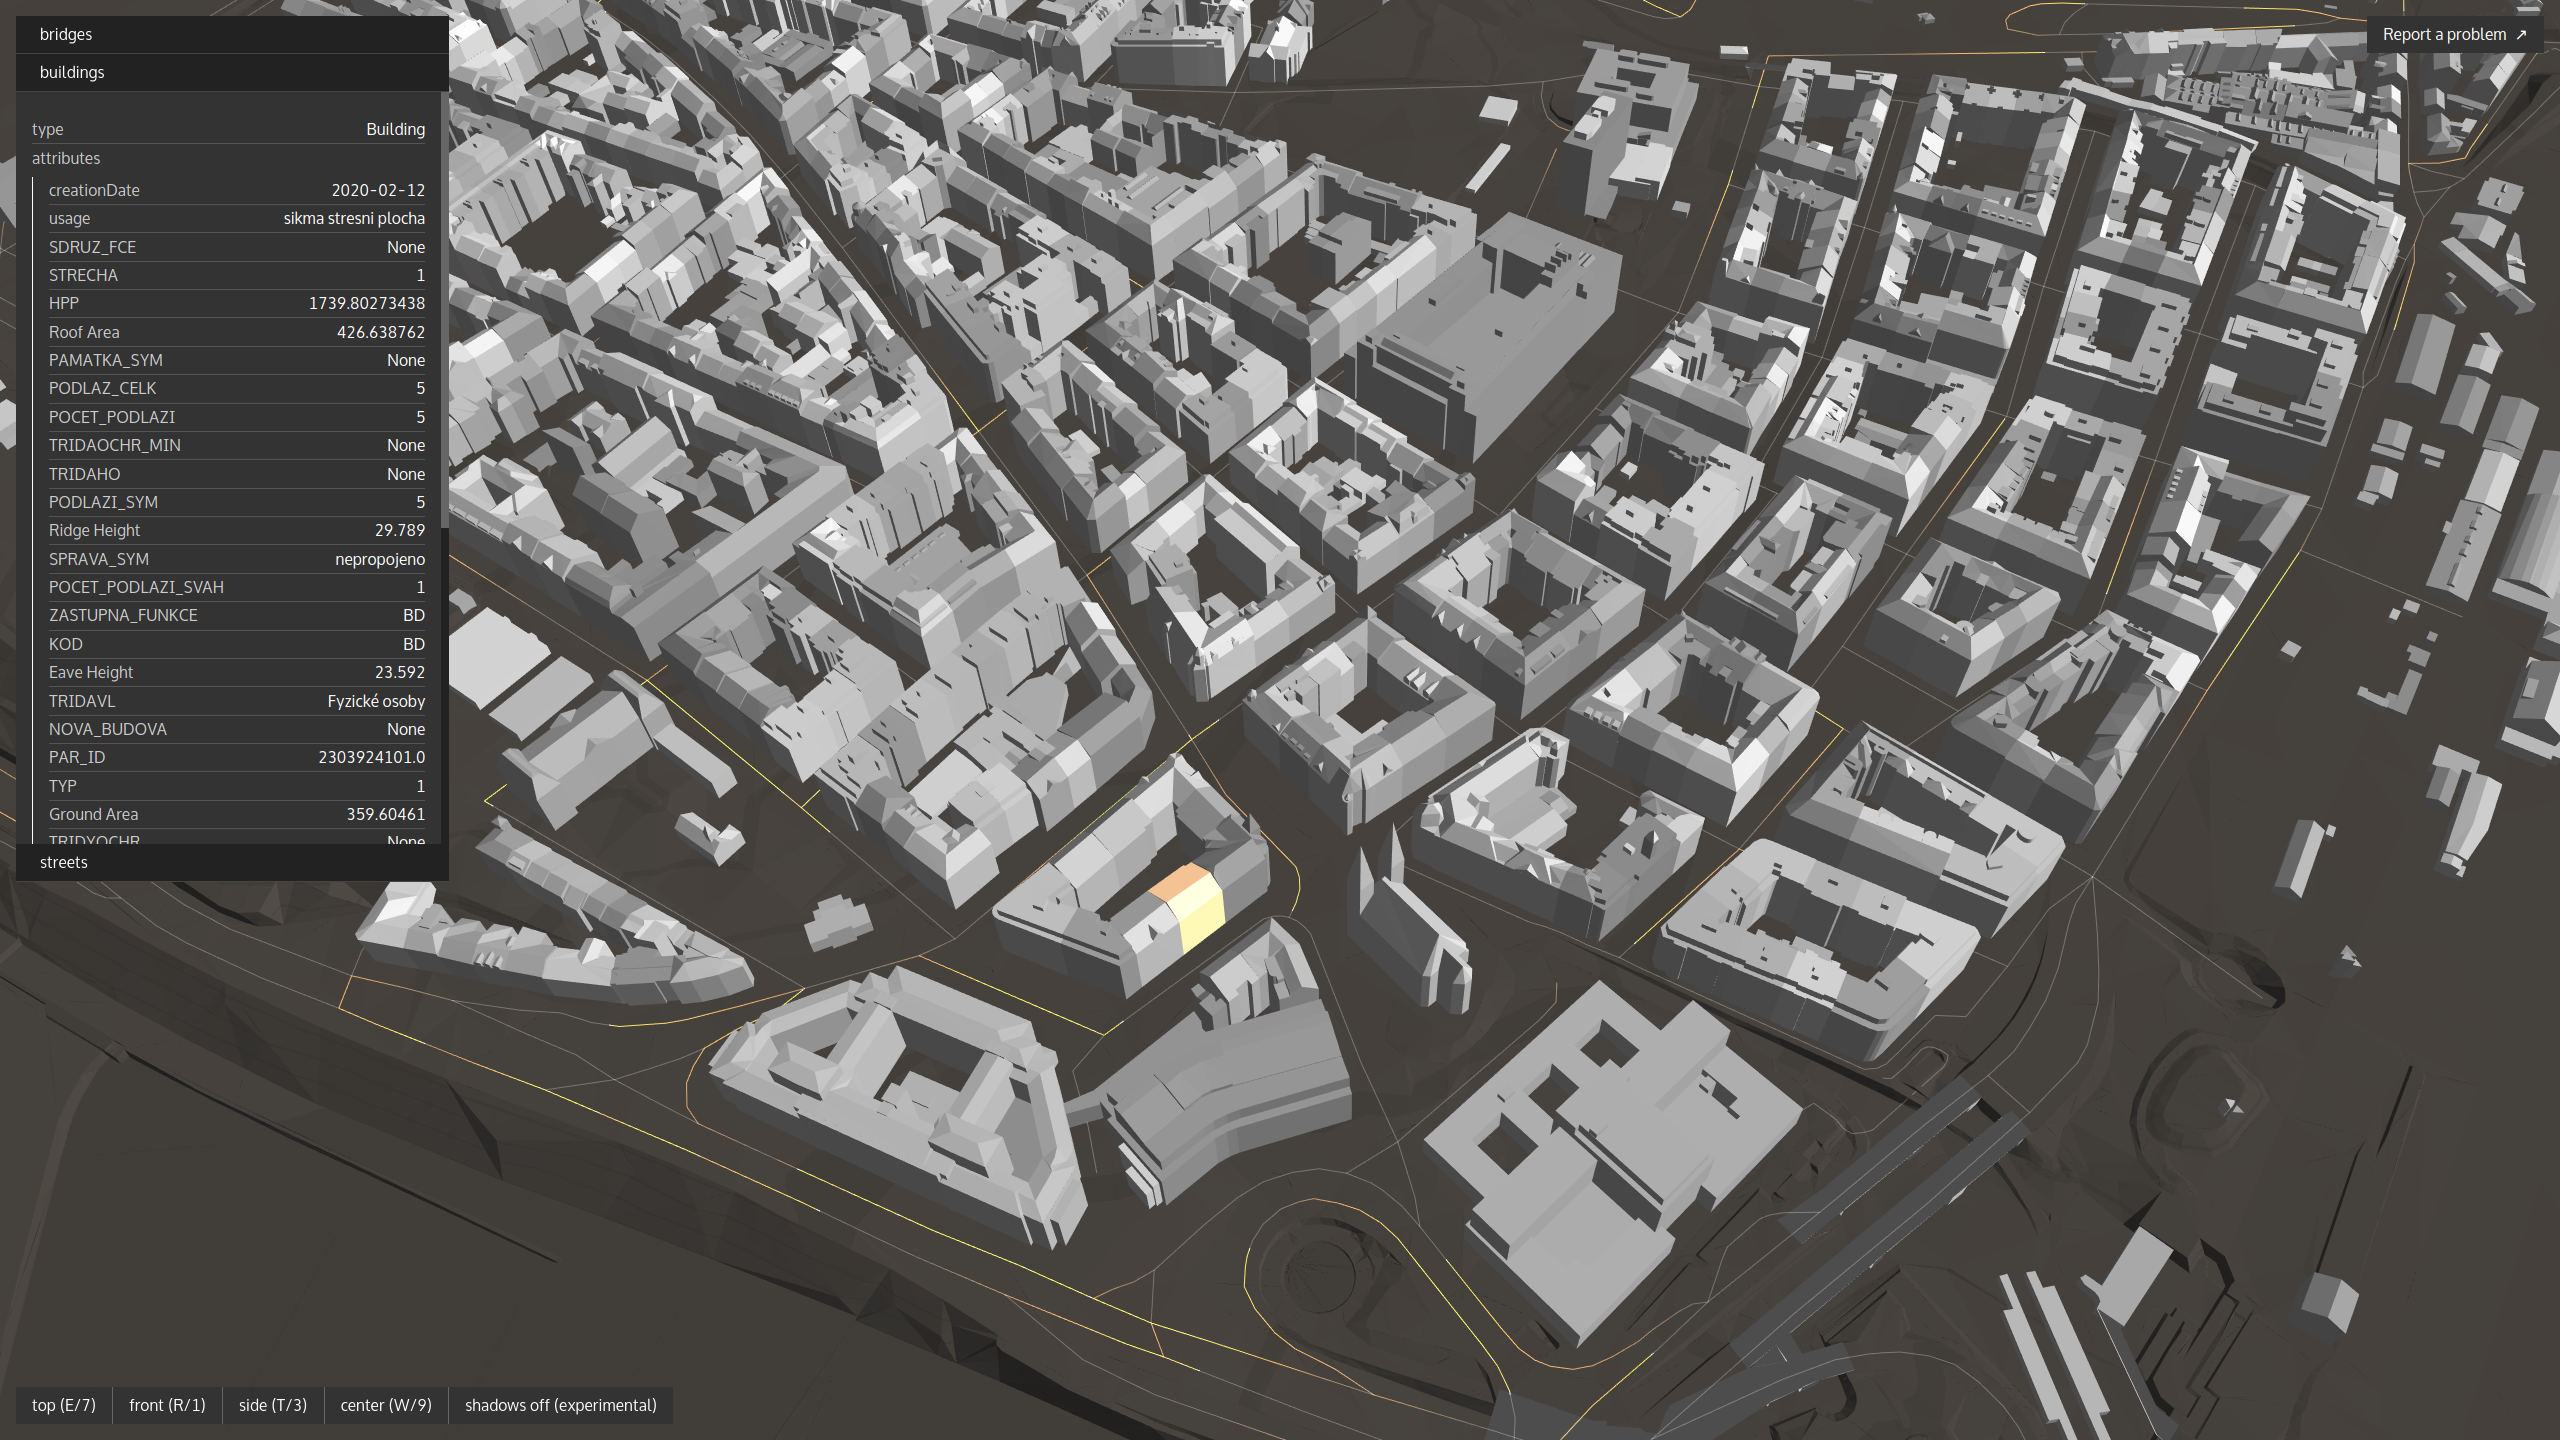
\includegraphics[width=1\textwidth]{imgs/metacity.png}
		\end{center}
	\end{frame}

	\begin{frame}
		\begin{columns}
			\begin{column}{0.5\textwidth}
				\begin{center}
					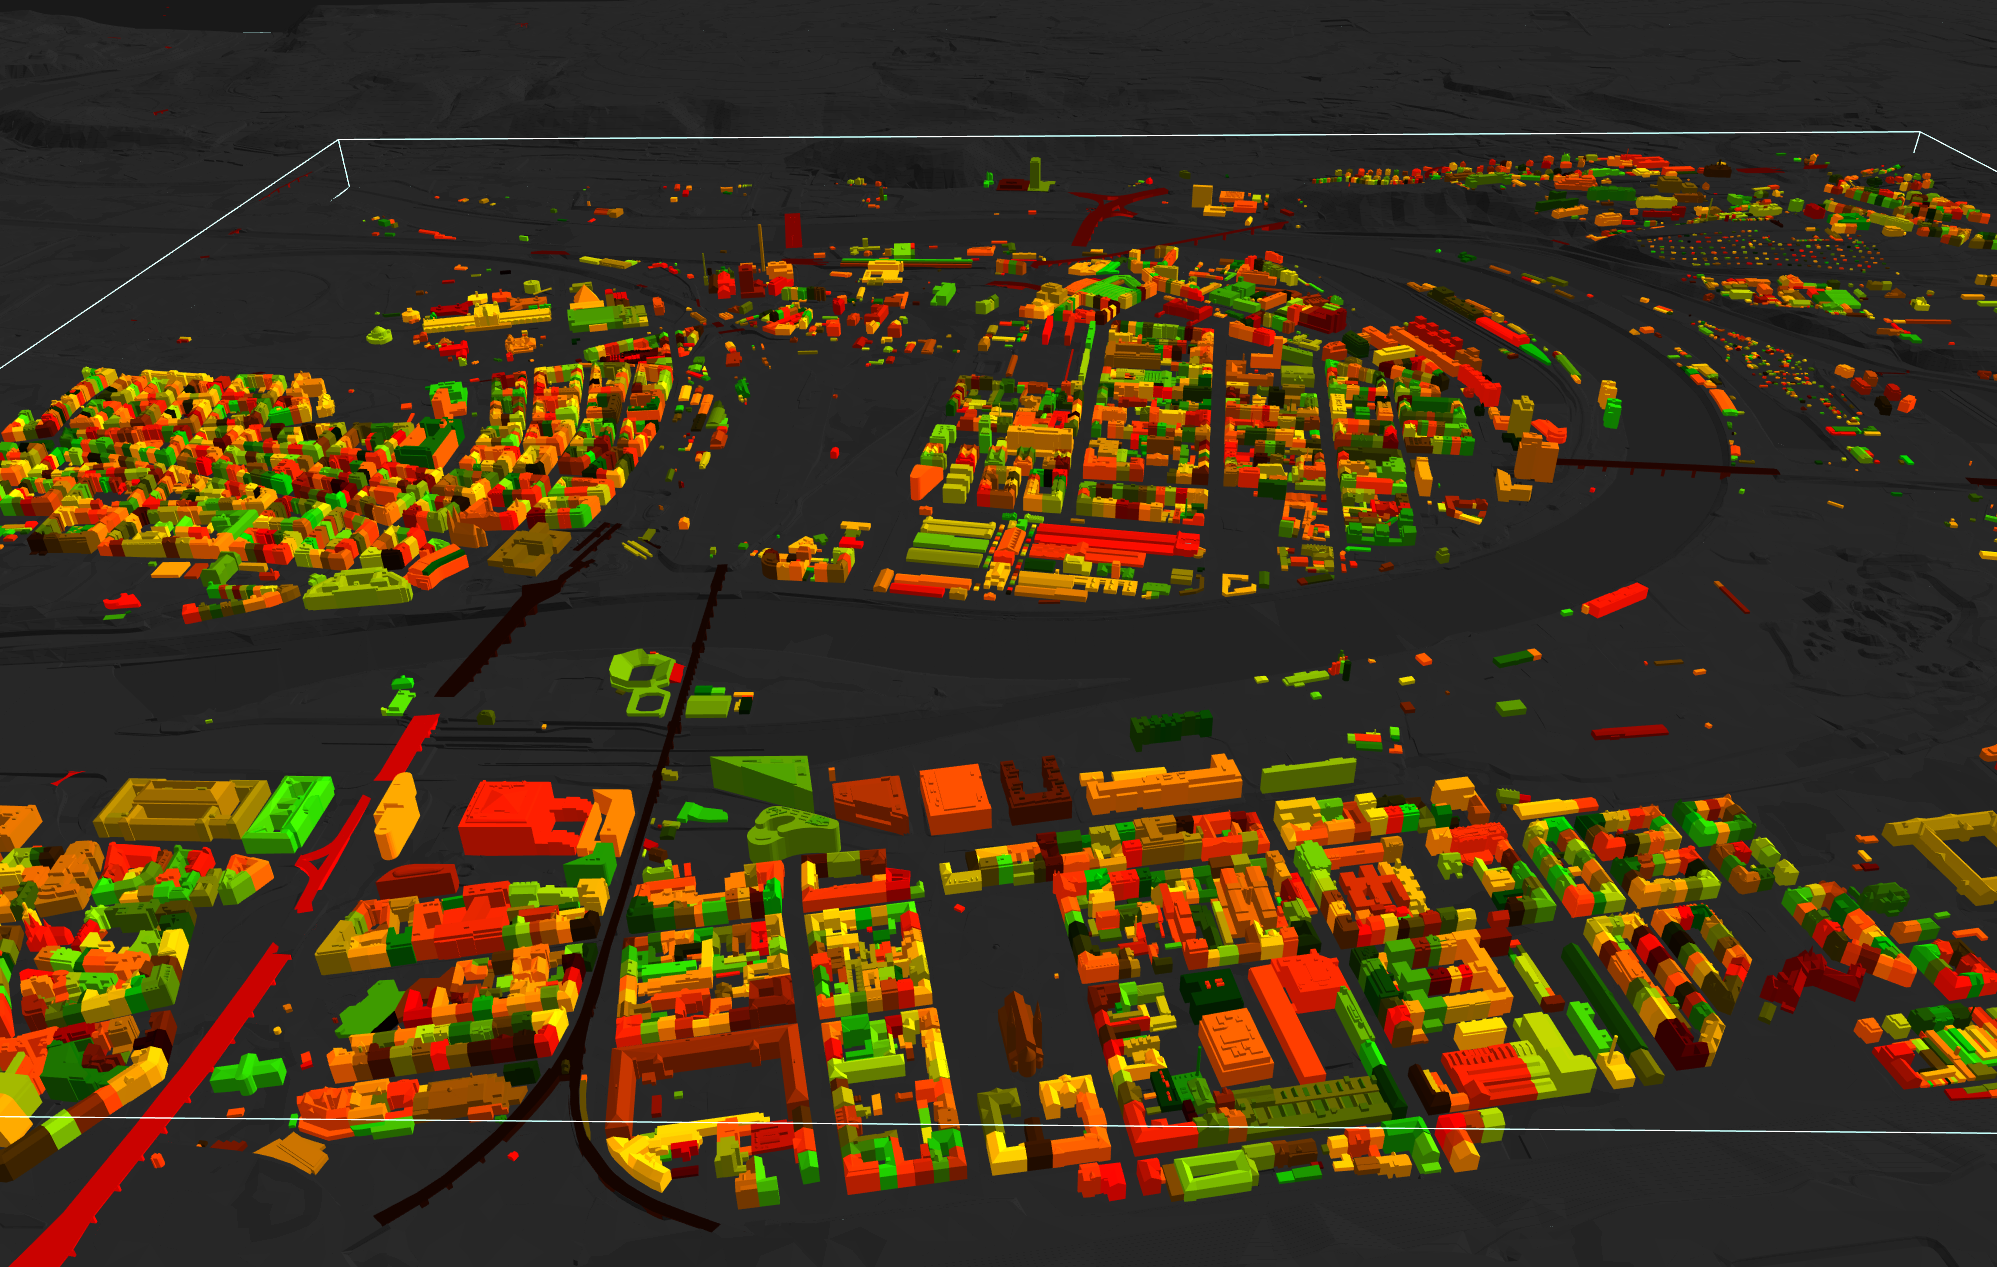
\includegraphics[width=1\textwidth]{imgs/metacity0.png}
				\end{center}
			\end{column}
			\begin{column}{0.45\textwidth}
				\begin{center}
					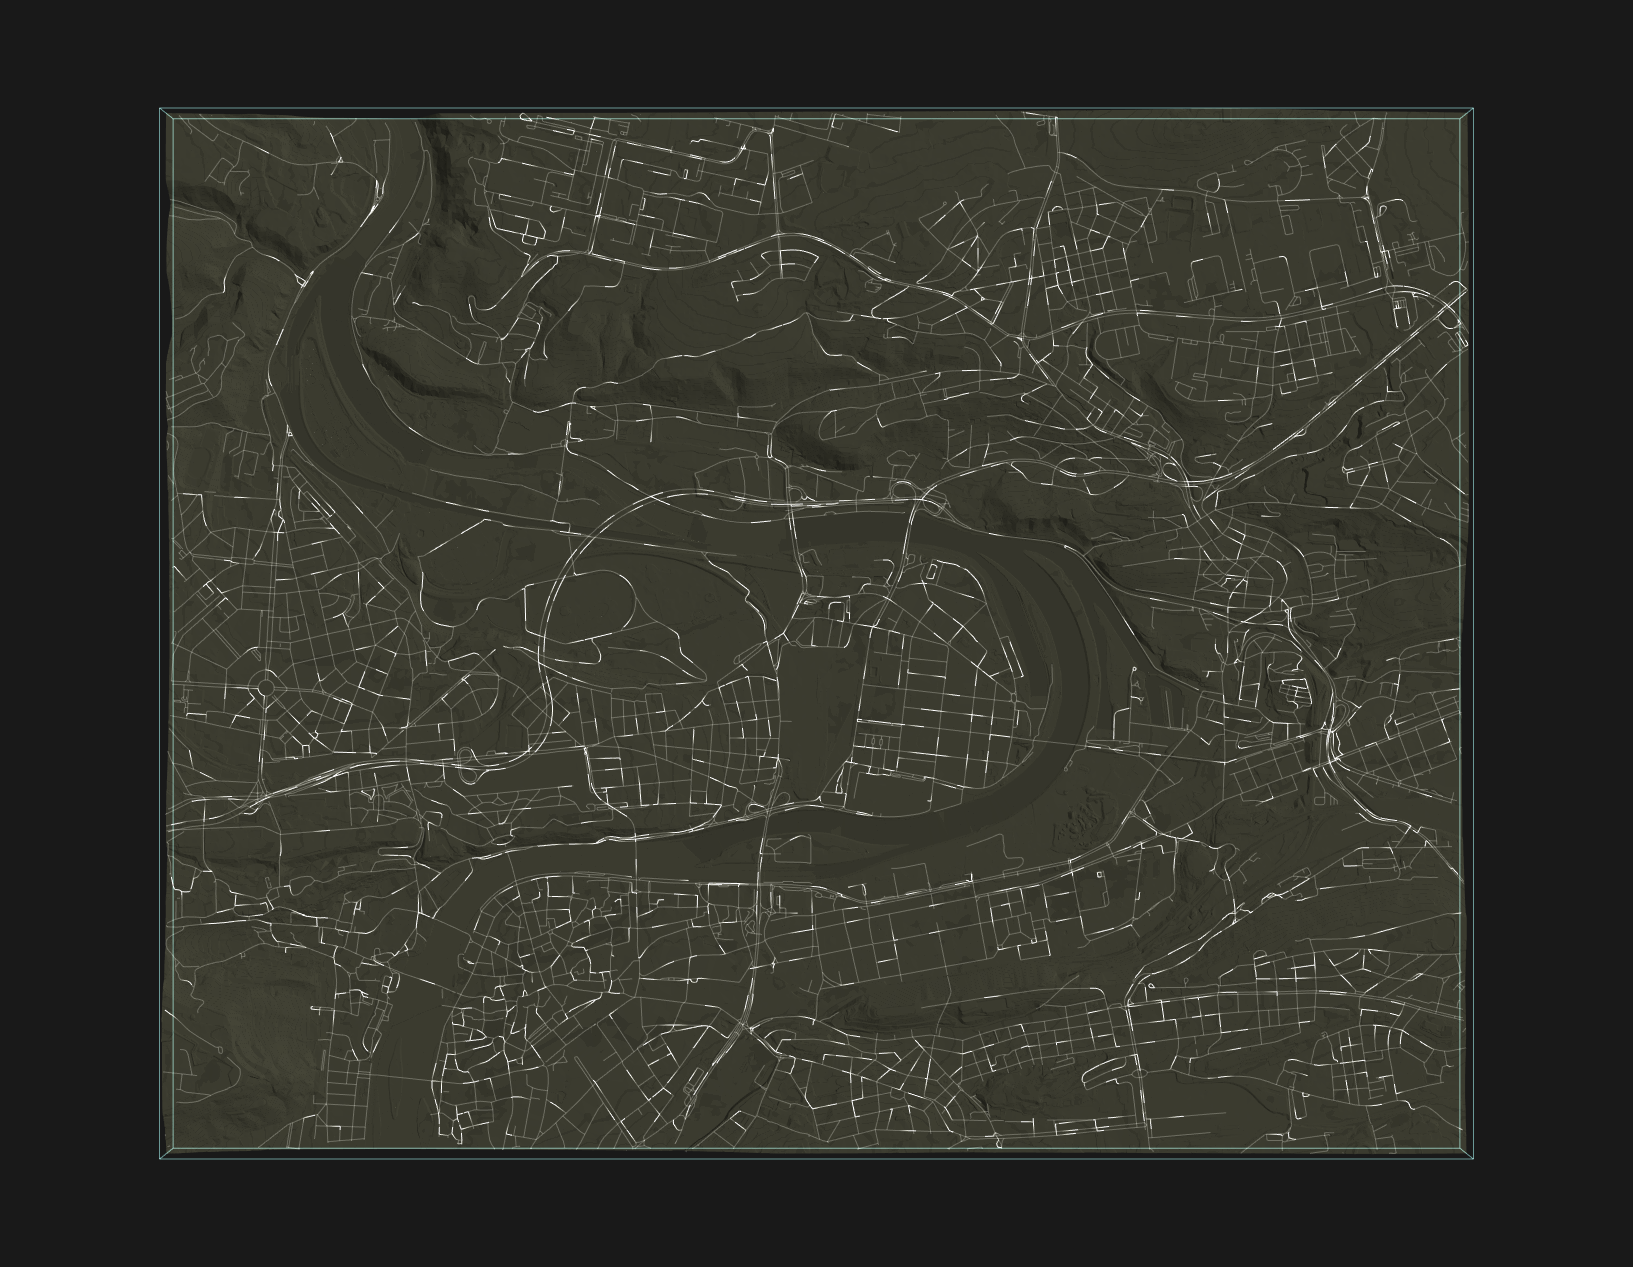
\includegraphics[width=1\textwidth]{imgs/webPrototype2.png}
				\end{center}
			\end{column}
		\end{columns}	
	\end{frame}

	\begin{frame}
		\frametitle{}
		\begin{center}
			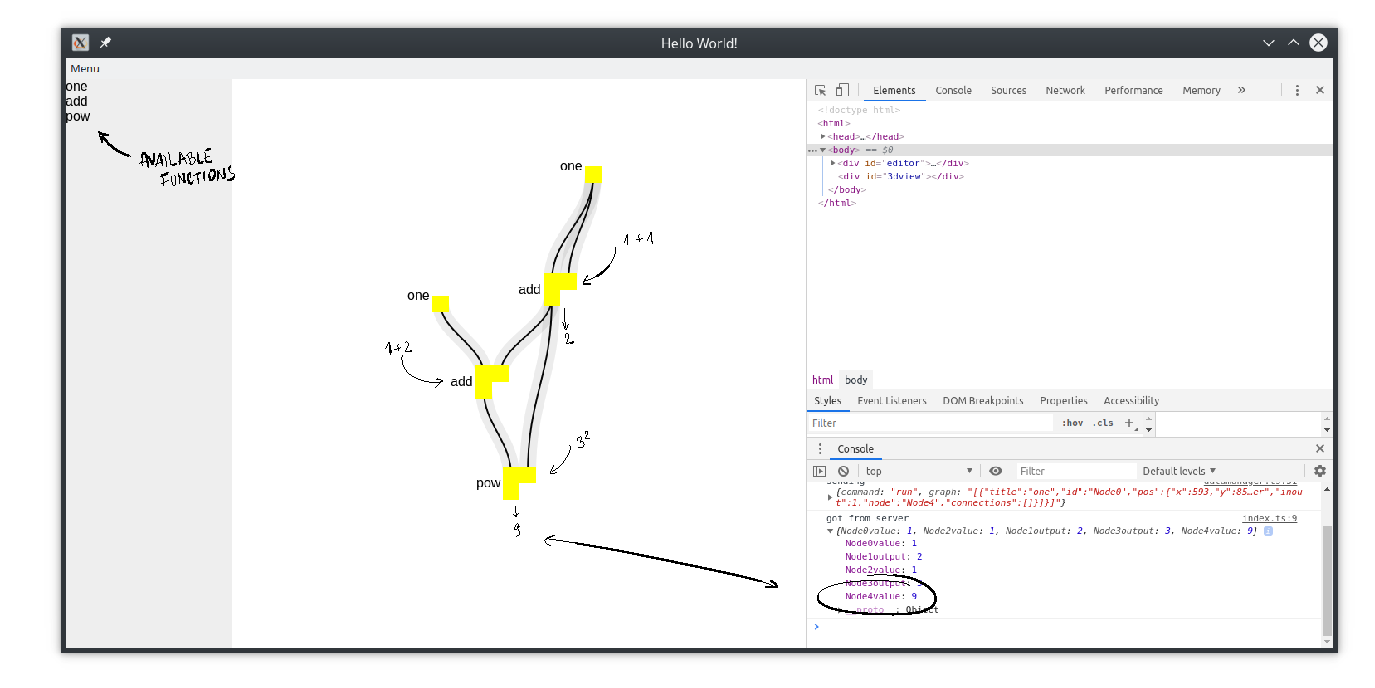
\includegraphics[width=1\textwidth]{imgs/editorDemo2.pdf}
		\end{center}
	\end{frame}

	\begin{frame}[fragile]
		Modularity and extensibility with Python plugins
		\begin{overprint}
			\onslide<1>
			
		\begin{minted}[
			linenos,
			numbersep=5pt,
			gobble=0,
			frame=lines,
			framesep=2mm]{python}
from parameters import param, output

@param('a', 'number') #(first input parameter name, type)
@param('b', 'number') #(second input parameter name, type)
@output('sum', 'number') #(first output parameter name, type)
def call(a, b):
    return a + b
		\end{minted}
		\end{overprint}
	\end{frame}

	\section{Conclusion}
	\begin{frame}
		\frametitle{Conclusion}
		\begin{itemize}
			\item visualization of urban data
			\item web-based solution --- editor and two viewers
			\item virtual tools with physical components
			\item physical components $\rightarrow$ accessibility, interactivity, playfulness\ldots
			\item two system modules created as a proof-of-concept 
		\end{itemize}
	\end{frame}

	\begin{frame}
		\frametitle{What is next}
		\begin{itemize}
			\item combine created POCs into a single framework
			\item data tiling and physical model assembly
			\item improve editor UI\ldots
		\end{itemize}
	\end{frame}


	\begin{frame}
		\frametitle{Sources}
		\tiny
		\textbf{Literature}
		\begin{itemize}
			\item Bits and Bricks: Tangible Interactive Matrix for Real-Time Computation and 3D Projection Mapping. I Winder, K Larson. Proceedings of the 2017 Future Technologies Conference (FTC), 2017
			\item Tang, L.; Chen, C.; et al. Building Information Modeling and Building Performance Optimization. In Encyclopedia of Sustainable Technologies, edited by M. A. Abraham, Oxford: Elsevier, 2017.
			\item Ledoux, H.; Ohori, K. A.; et al. CityJSON: A compact and easy-to-use encoding of the CityGML data model. Open Geospatial Data, Software and Standards, volume 4, no. 1, 2019
		\end{itemize}
		\textbf{Image Sources}
		\begin{enumerate}
			\item Ira Winder, MIT Media Lab, Big Data Analytics Tokyo 2017. In: YouTube [online]. 12. 5. 2017 [cit. 10. 9. 2020]. Available from: https://youtu.be/zVmc5\_KK5JU.	
			\item Tactile Matrix. In:Tactile Matrix [online]. Ira Winder, Andy Ryan, © 2013–2021. [cit. 10. 10. 2020]. Available from: https://ira.mit.edu/tactile-matrix. 
			\item Electronics components for Tactile Matrix. Drawing by Ira Winder. In: Tactile Matrix SDK [online]. Ira Winder, © 2013–2021. [cit. 10. 10. 2020]. Available from: https://ira.mit.edu/sdk.
			\item Rohanský ostrov: nový Karlín? Martin Vronský, IPR Praha, © 2020. [cit. 25. 11. 2020].	
		\end{enumerate}
	\end{frame}
	
\end{document}
